\mysection{System Performance Analysis}\label{performanceAnalysis}

Now we can analytically evaluate the given system performance model regarding various performance criteria using MPA.\
The main assignment will be to find out, whether the system-level timing properties of this specific implementation meet the specified timing requirements~\cite{wan:05}.
The exact analysis methods may slightly vary for different abstract components, but always remains deterministic.
Following, the performance analysis methods for a system out of GPCs are presented.

The reason why the following equations use the Infimum and Supremum, instead of just using the minimum or maximum, can be found in~\cite{cru}.
Both, the delay and the buffer space calculations, consider \(\alpha ^{u}\) and \(\beta ^{\, l}\),
as \(d_{\max}\) and \(b_{\max}\) occur whenever the maximum load of events arrives at the time of minimum resource availability.
Visually these sizes can be interpreted as \autoref{fig:delays-vis}.

However, the system performance model is able to provide even more insights to a system.
For example analyzing the characteristics of the outgoing service curves, can expose the individual utilization of resources.
Besides that, the throughput of the event streams can also be calculated quite easily using the data of the system performance model~\cite{wan:06}.

\begin{figure}
    \centering
    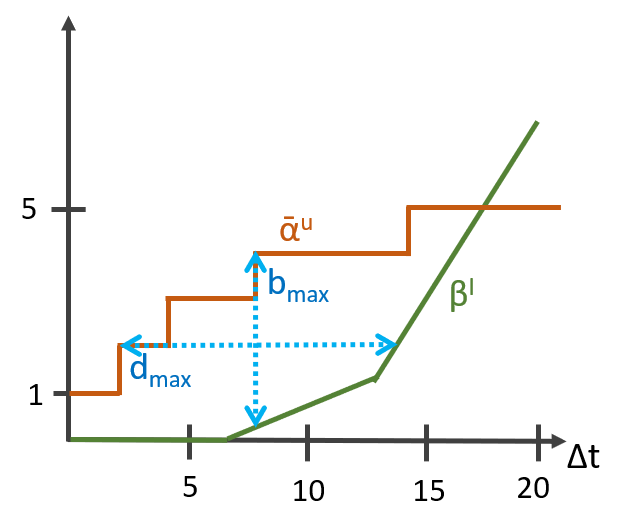
\includegraphics[width=0.7\columnwidth]{graphics/delays_vis.png}
    \caption{Graphically determining \(d_{\max}\) and \(b_{\max}\)}\label{fig:delays-vis}
\end{figure}

\mysubsection{Maximum Delay Guarantees}

The maximum delay \textbf{\(d_{\max}\)} experienced by any event on the event stream with arrival curve \(\alpha\) when being processed at a single GPC with service curve \(\beta\) is bounded by~\cite{cho:08}:
\[d_{\max} \leq Del (\alpha ^{u}, \beta ^{\, l})\]
\[Del (\alpha ^{u}, \beta ^{\, l}) := \sup_{\lambda \geq 0} \left\{ \inf_{\tau \geq 0}\left\{\alpha^{u}(\lambda) \leq \beta^{\, l}(\lambda+\tau)\right\}\right\}\]
The end-to-end delay experienced by an event with arrival curve \(\alpha\) that is being processed by \textbf{n} GPCs with the service curves \(\beta_{i}, \, i \in \{0, \ldots, n\}\) is furthermore bounded by:
\[d_{\max} \leq Del (\alpha ^{u}, \beta ^{\, l} _ 1 \otimes \cdots \otimes \beta ^{\, l} _n )\]
\[\leq Del (\alpha ^{u}, \beta ^{\, l} _1 ) + \cdots +  Del (\alpha ^{u}, \beta ^{\, l} _n ) \]
The calculation of the hard upper bounds to the maximum delays are quite conservative, yet they guarantee, that nothing every exceeds those bounds~\cite{cho:08}.

\mysubsection{Maximum Buffer Requirements}

We often also need to know how much storage space the internal buffers need, in order for them to always be able to temporarily store incoming events, that can not yet be processed.
This maximum required buffer space \textbf{\(b_{\max}\)} of a GPC with service curve \(\beta\) processing an event stream with arrival curve \(\alpha\) is bounded by~\cite{cho:08}:
\[b_{\max} \leq Buf \left(\alpha ^{u}, \beta ^{\, l}\right)\]
\[Buf \left(\alpha ^{u}, \beta ^{\, l}\right) := \sup _{\lambda \geq 0}\left\{\alpha^{u}(\lambda) - \beta^{\, l}(\lambda)\right\}\]
In the case of several consecutive tasks that all use the same shared memory, the required buffer space can be reduced to
\[b_{\max} \leq Buf (\alpha ^{u}, \beta ^{\, l} _ 1 \otimes \cdots \otimes \beta ^{\, l} _n )\] 
\[\leq Buf (\alpha ^{u}, \beta ^{\, l} _1) + \cdots +  Buf (\alpha ^{u}, \beta ^{\, l} _n ) \]

\mysubsection{Performance Analysis of the Sample System}

Both, architecture A and architecture B have the same buffer requirements.
In the sample system architecture A delays a brightness event by 50ms and a message event by 395ms.
Meanwhile, architecture B delays a brightness event by 40ms and a message event by 580ms.
As 580ms exceed the specified maximum delay of 500ms per message event, only architecture A is suitable for our scenario.